\documentclass[tikz]{standalone}

\usepackage{amsmath}
\usepackage{unicode-math}
\usepackage{mathtools}
\usepackage{derivative}

\setmainfont{Stix Two Text}
\setmathfont{Stix Two Math}

\usetikzlibrary{arrows.meta,fit,positioning}

\renewcommand{\familydefault}{\sfdefault}

% prefix equation numbers with section number
\numberwithin{equation}{section}

\DeclarePairedDelimiter{\ceil}{\lceil}{\rceil}
\DeclarePairedDelimiter{\floor}{\lfloor}{\rfloor}
\DeclarePairedDelimiter{\abs}{\lvert}{\rvert}
\DeclarePairedDelimiter{\norm}{\lVert}{\rVert}
\DeclarePairedDelimiter{\bra}{\langle}{\rvert}
\DeclarePairedDelimiter{\ket}{\lvert}{\rangle}
\DeclarePairedDelimiter{\expval}{\langle}{\rangle}
\DeclarePairedDelimiter{\norder}{\mathcolon}{\mathcolon}
\DeclarePairedDelimiter{\anorder}{\typecolon}{\typecolon}
	
\newcommand{\laplace}{\mbfnabla^2}
\newcommand{\trans}{{\scriptscriptstyle\mathsf{T}}}

\newcommand{\vdot}{\cdot}
\newcommand{\vcross}{\vectimes}
\newcommand{\vb}[1]{\symbfup{#1}}
\newcommand{\vu}[1]{\hat{\vb{#1}}}
\newcommand*\dd[2][\relax]{\mathop{\ifx\relax#1\odif{#2}\else \odif[order={#1}]{#2}\fi\,}}

\newcommand{\vacuum}{\ket*{\vb{0}}}

\DeclareMathOperator{\trace}{Tr}
\DeclareMathOperator{\sinc}{sinc}

\AtBeginDocument{
	\let\Re\relax
	\let\Im\relax
	\DeclareMathOperator{\Re}{Re}
	\DeclareMathOperator{\Im}{Im}

	\renewcommand{\div}{\mathop{\mbfnabla\vdot}}
	\newcommand{\curl}{\mathop{\mbfnabla\vectimes}}
}

\DeclarePairedDelimiterX{\comm}[2]{[}{]}{#1,#2}

\DeclarePairedDelimiterX{\braket}[2]{\langle}{\rangle}{#1\delimsize\vert#2}
\DeclarePairedDelimiterX{\ketbra}[1]{\lvert}{\rvert}{#1\rangle\delimsize\langle#1}



\usetikzlibrary{arrows.meta}
\usetikzlibrary{decorations.pathmorphing}

\begin{document}
	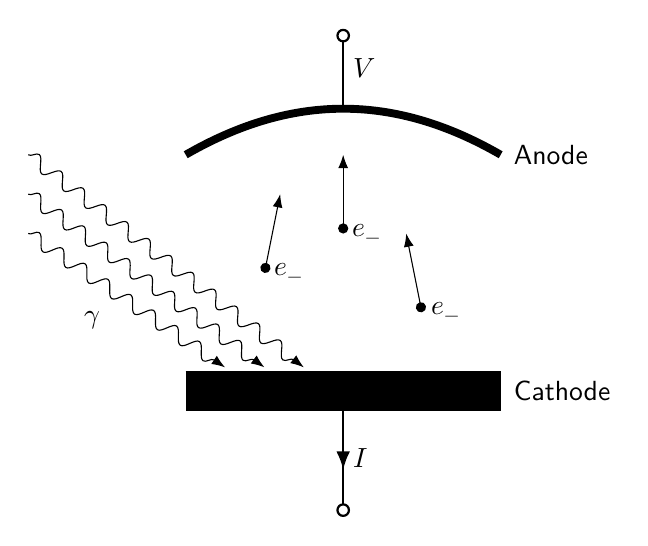
\begin{tikzpicture}[
		photon/.style={-Latex, decorate, decoration={snake, post length=1mm}},
		electron/.style={Circle-Latex},
	]
		\draw[line width=5mm] (0,0) -- ++(4,0) node[right, xshift=-0.2cm] {Cathode};
	
		\draw[thick, -Latex] (2,0) -- ++(0,-1) node[right, yshift=0.15cm] {$I$};
		\draw[thick, -{Circle[open]}] (2,-0.6) -- ++(0,-1);
		
		\draw[line width=1mm, bend left] (0,3) to ++(4,0) node[right] {Anode};
		\draw[thick, -{Circle[open]}] (2,3.6) coordinate (ca) -- ++(0,1) node[midway, right] {$V$};
		
		\draw[photon] (-2,2) -- (0.5,0.3);
		\draw[photon] (-2,2.5) -- (1,0.3);
		\draw[photon] (-2,3) -- (1.5,0.3);
		\draw (-1.2,0.9) node {$\gamma$};
		
		\draw[electron] (2,2) node[right] {$e_-$} -- ++(0,1);
		\draw[electron] (3,1) node[right] {$e_-$} -- ++(-0.2,1);
		\draw[electron] (1,1.5) node[right] {$e_-$} -- ++(0.2,1);
	\end{tikzpicture}
\end{document}
